\chapter{Estudio de Diagnóstico}

\section{Seguimiendo de la Pandemia}

A causa del COVID-19, a nivel global se han registrado aproximadamente 34 millones de personas contagiadas y 1 millón de muertes confirmadas hasta la fecha 1 de Octubre del año 2020,cuyo desenlace causa pánico y desorden público a través del mundo. La Organización Mundial de la Salud (OMS) declaró al COVID-19 como una emergencia de salud internacional, dando recomendaciones para prevenir y controlar el contagio de la misma. En Bolivia se tiene registrados 135,311 enfermos, de los cuales 7.965 han fallecido y 31.817 casos activos restantes, además de 95.529 pacientes dados de alta, dando al COVID-19 un ratio de mortalidad de 5,89\% en Bolivia. Eventualmente se tomaron medidas de prevención, las cuales son fuertemente criticadas independientemente de la calidad de resultados, siendo la principal la declaración de una cuarentena que ha impactado servicios de transporte, comercio, entretenimiento, educativo y muchos más; por lo cual se han estado viendo sofocadas las posibilidades de salir libremente y realizar actividades que solían ser consideradas como cotidianas.\\

Esta cuarentena implicó que las ciudades del mundo impongan nuevas leyes de confinamiento, implementando advertencias, multas y cárcel para quienes incumplan las mismas, así mismo, se cancelaron eventos festivos, se cerraron escuelas y pospusieron clases, incluso negocios que no eran considerados necesarios para la primera necesidad de la población tuvieron que cerrar temporalmente durante largo tiempo hasta que las personas adoptaron costumbres de higiene personal. El deporte ha sufrido especialmente debido a la influencia del COVID-19 como nunca antes ha acontecido, por ello las personas, especialmente los deportistas precisan de mantener sus rutinas diarias de ejercicio físico y las empresas deben planear nuevos modelos de negocio en orden de ajustarse a los cambios.\\

Se recomienda hacer ejercicio durante al menos 30 minutos cada día o al menos 20 minutos de exigencia vigorosa. En cuanto a niños, ancianos o enfermos crónicos, consultar con un medico es recomendado. Mantenerse en casa es efectivo para evitar la expansión de esta enfermedad, pero mantener la actividad física es un punto importante.\\

El ejercicio en casa puede realizarse de demasiadas formas y muy variadas, basta con buscar un ambiente que respete las medidas de prevención para el COVID-19 y sea un espacio mínimamente grande para moverse cómodamente con los brazos y piernas extendidos, aunque no sean de las mejores practicas, es incluso suficiente un metro cuadrado para entrenar en distintos deportes o disciplinas. Se pueden exhibir múltiples ejemplos de ejercicio, por lo que es casi imposible tener una excusa, la población que no puede darse el lujo de ejercitarse, esta en una situación deplorable económicamente, carece del tiempo debido a un exceso insano de trabajo, problemas de salud u otros.
Se pueden realizar entrenamientos desde flexiones, sentadillas, abdominales, trotar en el mismo lugar y hacer juego de pies, así mismo se puede practicar Yoga, Tai Ji Quan, Karate, Tae Kwon Do y diversas artes marciales que poseen técnicas y practicas tanto en ambientes grandes como pequeños y puede ser practicado en relativamente cualquier momento, solo con la presencia de voluntad y un tiempo bien administrado. Existen innumerables vídeos y guías de ejercicio para realizar en Internet y televisión e incluso juegos o aplicaciones para poder ejercitarse lo necesario o ir más allá.\\

Esto no significa que el deporte o el ejercicio deba ser obligatoriamente limitado o que se deben restringir si no se cumple con estas restricciones, sino que esta es una medida más en contra de la expansión del COVID-19 hasta que exista una vacuna o resistencia efectiva ante ella \cite{Chen}. \\

La tutoría de entrenadores a deportistas siempre ha sido a partir de ordenes y tutoriales cuya base teórica es el enfoque cognitivo (aprender procesando la información a partir de lo que vemos y adquirimos de esa experiencia). Esto significa que la experiencia personal y el entrenamiento previo o visualización de resultados de los entrenadores se verá reflejado en su metodología de enseñanza, señalizando principalmente ordenes de ejecución de movimiento, entrenamiento mental (cuyo objetivo es desarrollar la autoestima y pensamiento/visualización positiva) y la retroalimentación para corregir errores y perfeccionar la técnica\cite{raiola2017motor}. \\

\section{Investigación Sobre el Karate}

Entre las múltiples disciplinas y deportes que existen, se planifica trabajar con el arte marcial del Karate Shotokan, debido a varias razones que se explicarán a continuación, entre ellas su larga historia, su fundamento filosófico, la practica de posiciones y técnicas y finalmente, es vastamente practicado alrededor del mundo.\cite{Inti}.\\

El Karate-Do es un arte marcial japónes que usa patadas, puñetazos, rodillazos, golpes de codo, mano abierta, rodilla, etc. En si toda parte del cuerpo esta indirecta o directamentamente relacionada a su práctica. Se ramifica en tres tipos de prática, ya que esta tiene diferentes fines según se practica:

\begin{itemize}
	\item Arte: Unicamente la práctica tradicional que se enseña en escuelas antiguas, con el fin de vivir el día a día con su filosofía y acondicionamiento físico, para vivir una vida equilibrada.
	\item Defensa personal: Desarrollar técnicas y potenciar el desarrollo personal, se busca una preparación mental y física para ser agredido y responder en cualquier momento.
	\item Deporte de combate: Se desarrolla un criterio de karate trabajado en reglas y capacidades para evitar agredir directamente, se busca demostrar la perfección de las habilidades en público y ganar reconocimiento, actualmente la mayor parte de las escuelas en Cochabamba son parte de la organización departamental de Karate perteneciente a la World Karate Federation (WKF).
\end{itemize}

Este arte marcial marca una distinción entre la práctica como técnica y el desarrollo interior del practicante, por ello se divide en dos:

\begin{itemize}
	\item Do, que es interpretado como búsqueda espiritual, que indica que señala la búsqueda de la perfección individual como persona.
	\item Jutsu que significa técnica, la repetición continua de las mismas hasta llegar a la perfección en su ejecución.
\end{itemize}

El Karate-Do va más allá del conocido acondicionamiento físico, desarrollo técnico y táctico. Busca un equilibrio de cuerpo y mente, desarrollando ambos al mismo tiempo, creciendo tanto como persona como ciudadano ejemplar. Para lograr este objetivo se imparten principios y objetivos, entre ellos la humildad, coraje, honor, lealtad, imparcialidad y mas. Estos valores son transmitidos en todos los dojos a sus practicantes mediante un credo inculcado y explicado lentamente a lo largo del aprendizaje práctico del arte marcial. Desde un punto de vista externo, muchos de estos valores y aprendizajes son solicitados por empresas que buscan personal responsable para las empresas.\\

El Karate Shotokan es originario de Okinawa, creado por Gishi Funakoshi en el siglo XIX, el "padre del Karate moderno" o Karate-Do, así como otros estilos de artes marciales, esta influenciado por disciplinas de países como Tailandia, Filipinas e Indonesia. En el año 1891 la prohibición de las artes marciales en Japón fue abolida, Funakoshi consolido una escuela con muchos estudiantes a finales del año 1910 , 20 años después, tras mucho esfuerzo, Funakoshi dirigía una docena de dojos universitarios. En 1947 tras la prohibición de artes marciales de la segunda guerra mundial, la Japan Karate Association (JKA) nombre a Funakoshi como el jefe instructor de la organización, dando lugar al Karate Shotokan como el más practicado en Japón, dirigiéndolo hasta el día de su muerte el 26 de abril de 1957 \cite{diez2012karate}.\\


Funakoshi, estudiaba la filosofía del Confucionismo, influyendo vigorosamente en la filosofía del Karate Shotokan. Una curiosidad es el significativo nombre del estilo Shotokan, dividido entre "Shoto" o más bien "Pino que se balancea" y "kan" que es escuela, casa o salón, Shoto era también el seudónimo que usaba el maestro Funakoshi para firmar su poesía, este nombre viene de la paz que le traía a Funakoshi el pasear por el bosque, afirmando ser parte de su rutina que le traía paz espiritual. \\

El Karate Shotokan es un estilo del Karate-Do, que esta caracterizado por ser súbito y explosivo, evitando la oportunidad de bloquear o contraatacar, sin embargo, para culminar este resultado es necesario sentar las bases de estas técnicas y posiciones para poder ejecutarlas con velocidad. Previo a practicar con velocidad y fuerza esta técnica, se necesita practicarla lentamente para entender el posicionamiento del cuerpo.\\

La práctica seria de este arte marcial emplea la metodología de enseñanza del método "Kaizen" o mejora continua, que involucra una capacidad de repetir miles de veces cada técnica y posición que existe en la búsqueda de perfeccionarla, siendo una meta inalcanzable, ya que al rozarla, uno entiende lo lejos que se encuentra. En el proceso de entrenamiento se denotan dos particularidades, la velocidad en que se realizan los movimientos y las pausas que hay entre las técnicas.\\

Esto es especialmente notable en los niños, en su mayoría pierden el interés tras la introducción del método Kaizen a ellos, la continua repetición de cada técnica es insoportablemente aburrido, sin mencionar el rigor del entrenamiento, las expectativas van subiendo cada vez que mejoran, por lo que pueden aplastar a los practicantes  \cite{o1999students}.\\


El Karate Shotokan tuvo múltiples oportunidad de crear un reglamento solido por parte de los universitarios que pertenecían a clubes universitarios, para que en 1957, año en que fallece Funakoshi, se celebro la primera Competición Nacional Universitaria de Karate de Japón \ref{jkachamp}.

\begin{figure}[t!]
	\centering
	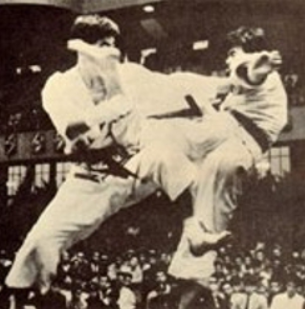
\includegraphics[width=8cm,height=5cm,]{./Images/1stJKAChampionships1957.png}
	\caption{Primer Campeonato de la JKA en 1957}
	\label{jkachamp}
\end{figure}

El año 1964 se crea oficialmente la Federación Japonesa de Karate-Do (JFK), una organización que une a diferentes estilos de Karate. El año de 1970 se crea en Japón la Federación Internacional de Karate (WKF) para unificar las Federaciones continentales, sus escuelas y competidores bajo un solo reglamento que es actualizado cada año desde entonces bajo el concepto del Karate, solo cambiando para mejorar continuamente. Posteriormente en el año 1990 se funda la Federación Mundial de Karate (WKF) bajo las mismas siglas, con 173 federaciones participantes y cuyo objetivo es que el Karate Deportivo sea reconocido como un deporte olímpico. Esta meta suponía iba a ser lograda el año 2020 en las Olimpiadas de Tokyo, cuyo debut fue irrumpido por la pandemia provocada por el COVID-19. En Bolivia, este arte marcial fue introducido en Bolivia por Freddy Escobar  el año 19XX\cite{Inti}. \\

En Bolivia, los actuales representantes de la practica como el Shihan Freddy Escobar, el Sensei Inti Escobar, Fernando Sugiura, Eddy Beltrán y más maestros sobresalientes colaboran para expandir su conocimiento a través de escuelas de Karate solo en Cochabamba.\\[1cm]


\subsection{Karate en Tiempos de Pandemia}

El Karate Shotokan emplea el cuerpo como un arma, cada parte del cuerpo se convierte en una, pero para dominar una técnica, se requiere de una técnica de respiración que permite proporcionar mayor fuerza, sin embargo, esta técnica es diferente a respirar, ya que se tiene que hacer violenta y profundamente, como si uno se encontrara trotando por largo tiempo, se tiene que utilizar constantemente para cada técnica que se usa en el Karate, desde el cambio de posición, golpear o simplemente respirar mientras se esta practicándolo, siendo este un factor de alto riesgo de contagio de COVID-19. \\
Los gimnasios de artes marciales son también afectados por la pandemia, por lo que cerrar fue su única alternativa hasta que las personas se ajusten a la nueva normalidad, en Cochabamba, "Bueno, la seguridad de los niños va primero, así que los mandamos a quedarse en casa, pero ahora en mes de octubre vamos a abrir una vez más con el nuevo reglamento de bio-seguridad e higiene para poder entrenar nuevamente"\ref{claseenPandemia}, dice Inti Escobar, Maestro de la Academia Bushido Kai  Desde Marzo, rápidamente Inti Escobar ha impartido clases online en la plataforma de Zoom para sus estudiantes \ref{clasevirtual} y así no perder el ritmo, pues es un entrenador de niños y adolescentes de Karate Deportivo, .

\begin{figure}
	\centering
\begin{subfigure}{.5\textwidth}
	\centering
	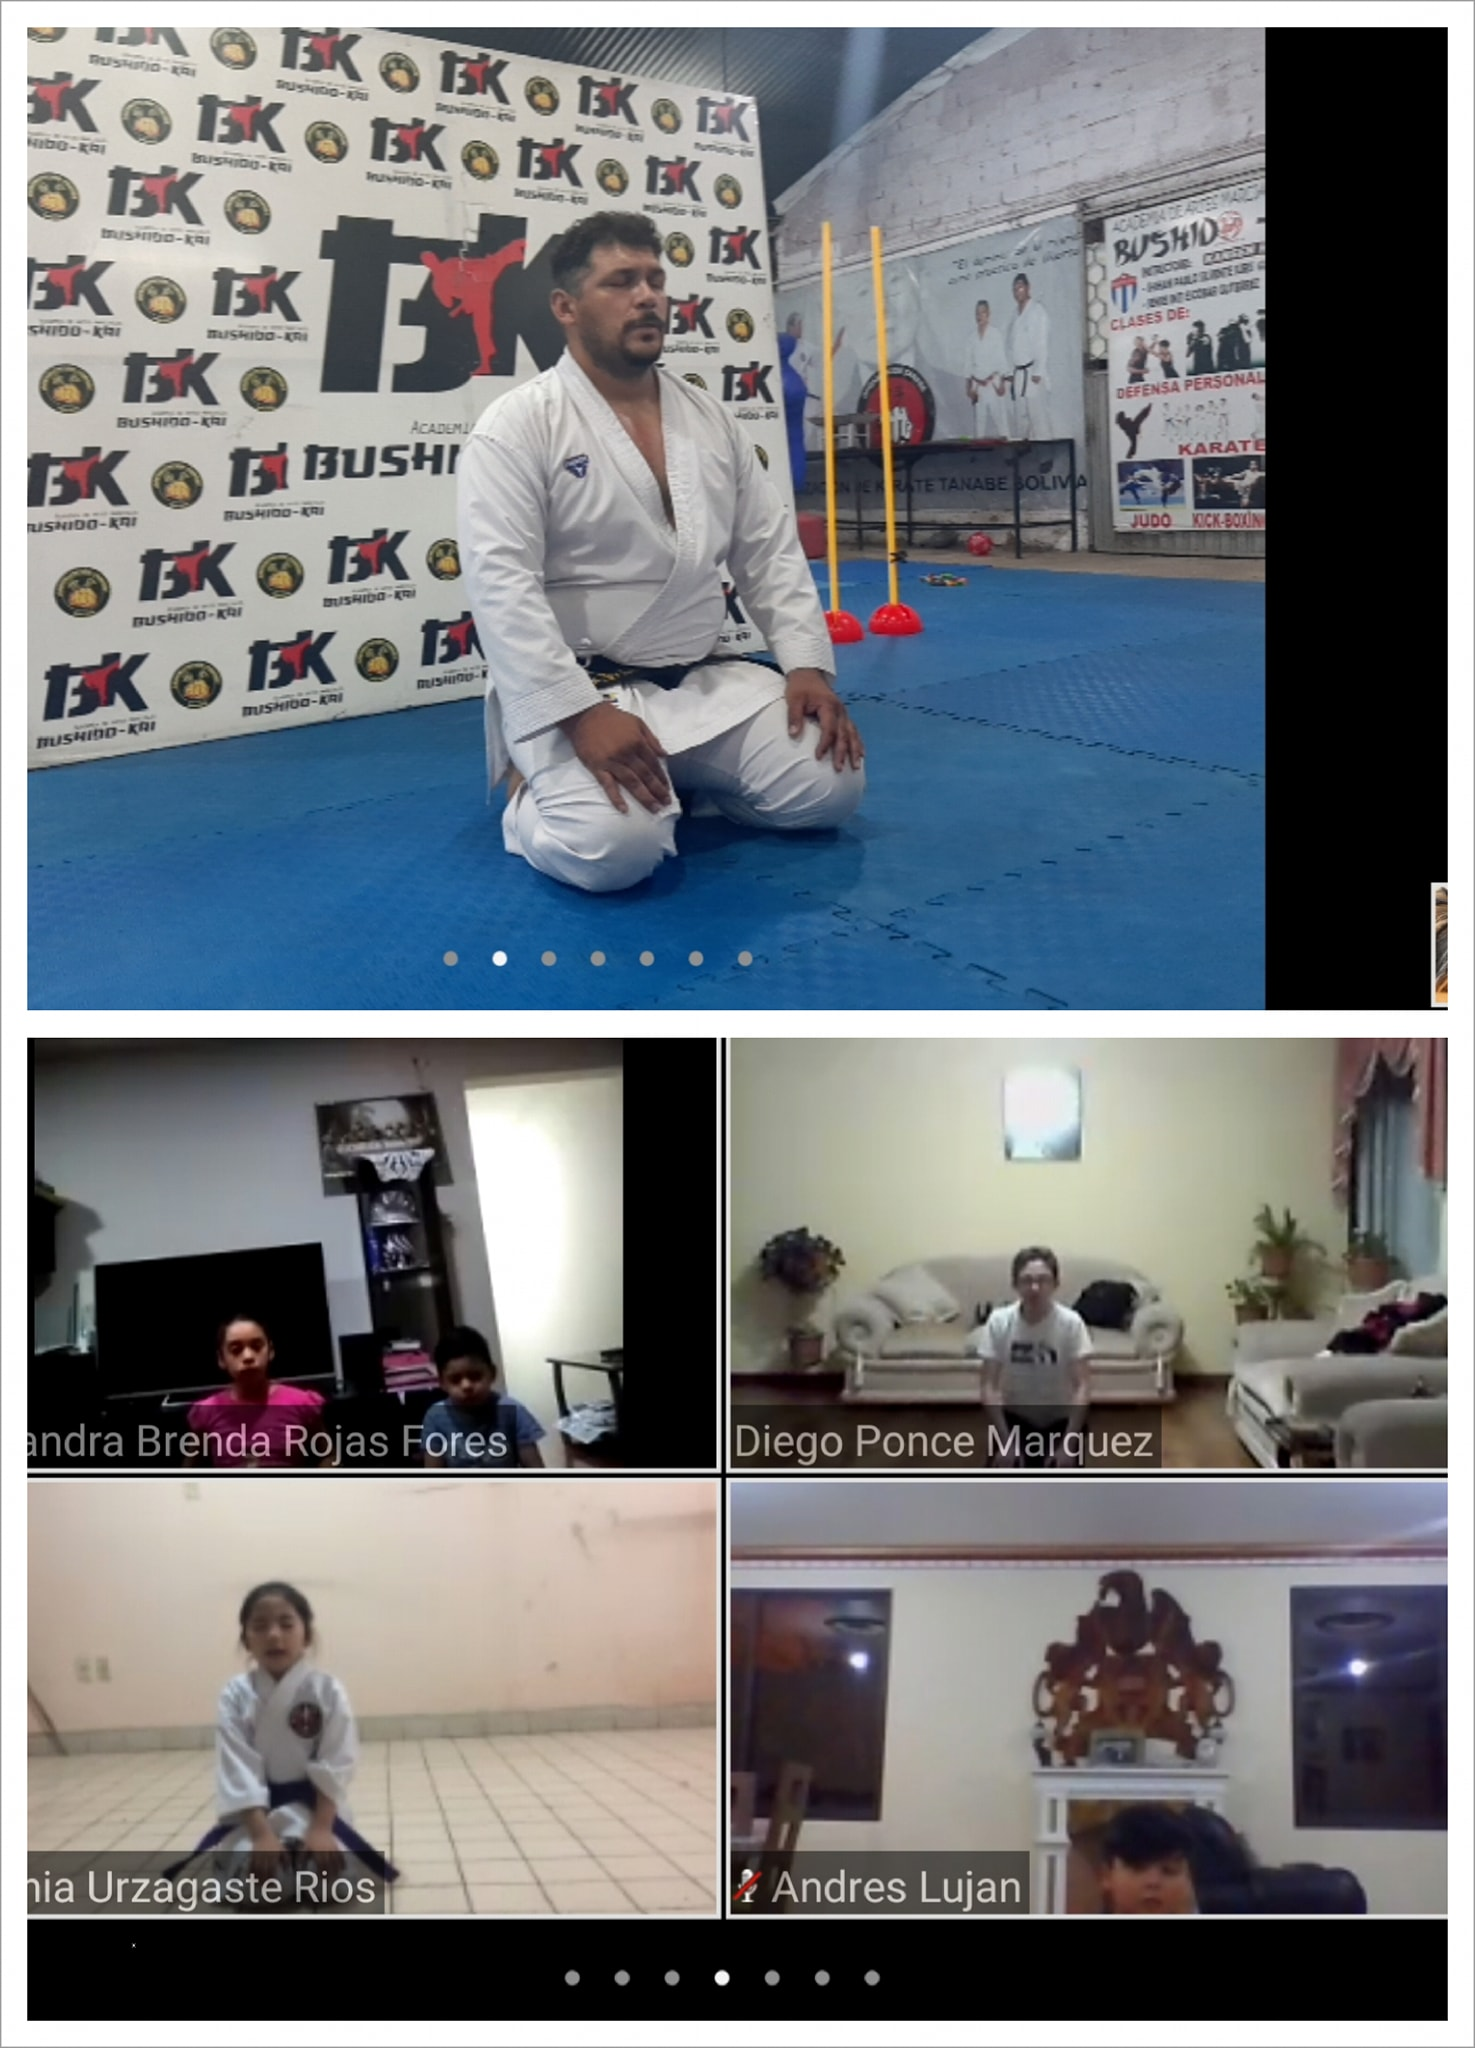
\includegraphics[width=8cm,height=5cm]{./Images/ClaseVirtual.jpg}
	\caption{Clases Virtuales}
	\label{clasevirtual}
\end{subfigure}%
\begin{subfigure}{.5\textwidth}
	\centering
	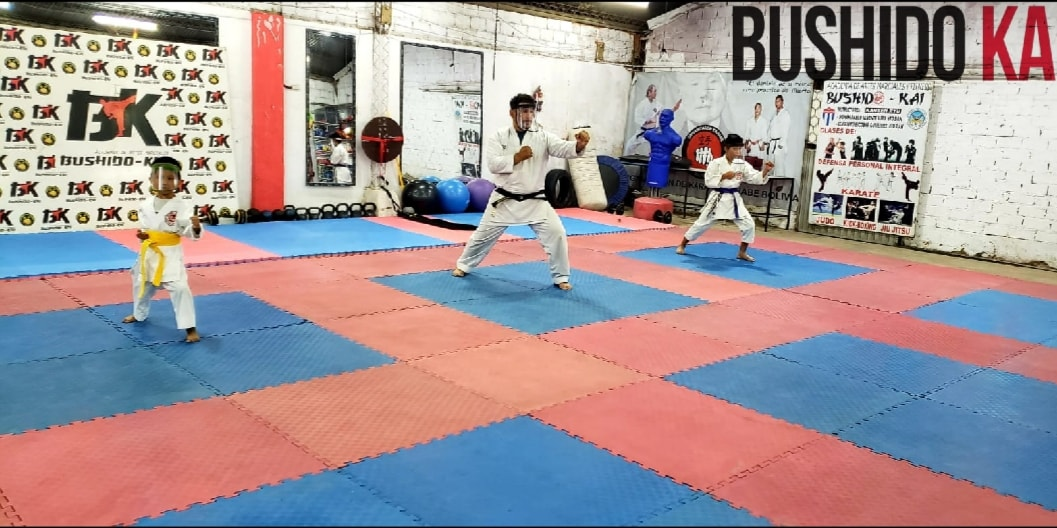
\includegraphics[width=8cm,height=5cm]{./Images/ClaseEnPandemia.jpg}
	\caption{Clases de Karate Con Medidas Para la Pandemia}
	\label{claseenPandemia}
\end{subfigure}
\caption{Karate Clases con Medidas de Bio-Seguridad}
\label{karateclass}
\end{figure}



2.- Esta propuesta nace del Sensei Inti Escobar, que dirige el Dojo Bushido Kai de Cochabamba, consiste en  Recreación de un torneo de Karate no viable, por que
3.- Respuesta sencilla es sí, pero es mucho más complicado que eso, después de investigar un poco, se plantea el uso de controles con sensor de movimiento, sin embargo, la disponibilidad y los precios dificulta su alcance, ademas que pueden no soportar los movimientos bruscos.
4si .- Debido a esto se plantea el uso de cámaras o Kinect, sin embargo, kinect es un equipo caro que no tuvo grandes éxitos, por lo que es normal que nadie vaya a usarlo, así que se plantea el uso de cámaras normales
5.- Esto es importante ya que karate tradicional guardado en tecnologia es necesario para conservar la cultura y expandir sus horizontes y posibilidades

















